\documentclass[11pt,a4paper]{article}

\usepackage{fullpage}
\usepackage{listings}
\usepackage{graphicx} %images
\usepackage{array}
\usepackage{centernot}
\usepackage{hyperref}
\usepackage[margin=0.75in]{geometry}
\lstset{language=sh,basicstyle=\ttfamily}
\graphicspath{ {./images/} }
\newcolumntype{C}[1]{>{\centering\arraybackslash}p{#1}}

\newcommand{\cmd}[1]{\texttt{#1}}

\begin{document}
\title{The WACC Compiler Report: Group 22}
\author{
Luke, Tan \\
\texttt{lt1519@ic.ac.uk}
\and
Richard, Yang \\
\texttt{ry819@ic.ac.uk}
\and
Zirun, Zhai \\
\texttt{zz4319@ic.ac.uk}
\and
Jia Qi, Poon\\
\texttt{jqp18@ic.ac.uk}
}

\maketitle

\section{The Final Product}
In this section we will be mainly focusing on the base WACC compiler we have worked on during the frontend and backend tasks as functionality added in the extension will be addressed in a later section. 

\subsection{Functional Specification}
We are confident that our WACC compiler meets the functional specification of the project as per the specifications. This is because in addition to our code passing all of the required tests on LabTS, we also made sure it passes the advanced tests locally as well as various edge cases we came up with during production. 

\subsection{Performance Characteristics}
Performance-wise, we can consider the number of passes over the source file, the quality of the error messages and the quality of the assembly code. We pass over the source file a total of 5 times. Firstly, we pass through the source code twice during lexing and parsing using ANTLR to generate a ParseTree. Next, we use our visitor class to visit the ParseTree , performing the semantic checks and generating the AST. After that we traverse the AST to perform code generation using our translate function and finally build the output string by traversing the list of instructions and write to file in our Frontend and Backend classes.

The area that makes our compiler stand out would be the high quality of the error messages which we based off the Java JDK. We attempted to provide as much information to the user as possible - through a multitude of features.Firstly, whenever there is a syntax or semantic error, we will print the line number and highlight it with carets underneath to indicate where the problem occured. This is combined with specific error messages like incompatible types to aid the user.Instead of halting after a single semantic error, we continue on in order to flag out all the semantic errors at once. If however, multiple semantic errors occur on the same line, we would only print the first encountered error. For example, for the statement \texttt{bool b = 1 + "string" \&\& ‘c’ + true}, only the first assignment will be flagged out. Additionally, we added support for suggestions for common mistakes, like using single instead of double quotation marks to enclose a string.

As for the quality of assembly code, we do not have a reliable method of quantifying the quality since we are unable to consider run time on its own since execution time also includes the code generation and cross compilation. We did however try to model our assembly code after the provided WACC reference compiler and for the provided test cases they produce almost identical assembly code. 

\subsection{Basis for Future Development}
We took special care in ensuring that our code has a sound basis for future development by focussing on scalability and extensibility in our classes. Through extensive use of inheritance in AST Nodes, Types, Operands, Identifiers and Instructions, we made it easier to add new features to our compiler in the future as we could simply create a new class that extends the parent class and implement its abstract methods. 

Through the use of the ANTLR tool, any changes to the syntax and semantics can also be modified through the addition or modification of the autogenerated visit functions. Due to our clear separation of concerns regarding tokenization, parsing, semantic analysis, code generation and writing to file, we are also able to work on each individual concern separately without affecting the entire infrastructure. 


\section{Project Management}
\subsection{Coordination and Group Structure}
Our group was structured in a way such that we were all able to work separately through careful allocation of work and effective communication. At the same time, through the use of online calls and in person meetups, we were able to discuss important design details as a team. 

Due to the nature of our implementation, after the ParseTree was generated, we could do the various visit and check functions separately for each individual ParseTree and AST node. We branched out into our individual branches on git and only merged to the main task branch when we have successfully implemented and tested our code to allow us to work in parallel. 

We used a Google document to keep track of all the nodes that needed to be implemented and split them into different related subgroups such as Assignment and Variable nodes where it made more sense to be done by the same person. The Google document allowed us to keep track of what other members are working on to avoid clashes. It also made it easy for us to seek clarification on certain implementations as we could approach the person who did the task directly.

\subsection{Reflections}
Due to the level of trust between group members and our individual work ethic, we didn't have much allocation and instead relied on the proactiveness of each member to work on any unfinished task on their own. We had a Microsoft Teams meeting every few days to raise any issues and review our tasks. For smaller issues or clarifications as well as coordinating meetings, the Whatsapp group was used instead.     

The fact that all our group members lived in close proximity combined with the containment of the pandemic in Singapore meant that we had the luxury of in person meetups which made communication and discussion much more effective. 

On the other hand, I felt that we could have managed our timeline better. For all the different tasks, we usually left the bulk of the work to the final week where we had to work overtime. Since there was little buffer between tasks, we often took the first week of the new task to recuperate and catch up on our other courses just for the cycle to repeat again for the new task. In hindsight, these could have been avoided if we started work on the first task earlier and could have saved us a few late nights nearing the deadlines.


\section{Design Choices and Implementation Details}
\subsection{Language and Tools}
We decided to use Java as our implementation language mainly because of our familiarity with the language having used it in first year and in the Software Engineering Design Course. As a bonus, it is compatible with ANTLR and is the language of choice for most of the Teaching Assistants which ensures us access to more support. 

We used ANTLR as a tool for generating a ParseTree as it greatly simplified our task of creating a lexer and parser. Another particularly helpful feature was the autogenerated visitor class which provided a template for us to start our frontend.

To aid in our development, we used Gradle to auto-generate ANTLR files, compile source files and run tests. It has good support (in the form of plugins) for ANTLR and JUnit5, can handle dependencies easily, and eliminates the need to manually update our Makefile whenever we added new classes. For our testing, we used JUnit5 to run and organise our tests, making use of features such as tags which allows for selective testing, as well as the auto-generated XML test report to track our progress, since it can be directly read by Gitlab-CI and integrates well into our pipeline. Additionally, we used Docker to handle cross-compilation and emulation, which was convenient as we could avoid installing dependencies on every member’s computer, making it easier for the team to run the tests.

\subsection{Design Issues}
The two main design issues we faced were regarding register and AST  representation. For registers, we decided that since we want dynamically allocated registers, any node should be able to call a \cmd{getFreeRegister} function and receive a free register. We decided on a bitmap-like representation similar to Pintos frame allocation while abstracting away the handling of freeing and getting registers to the context class. This helps us separate the functionality so that when we want to change our register implementation we just have to make changes in a single class.  In the special case when we run out of free registers and data needs to be pushed to the stack, we decided to just return the last register which happens to be register 10. It is then up to the \cmd{binOpNode} to infer that if both expressions are stored in register 10 the first one must have been pushed to the stack. 

For the AST, we decided to separate the creation of the node, the semantic checking and the code generation into distinct functions. This is for clarity which helps us find the source of the problem during debugging. During creation, we do only the necessary checks required to create a well formed node. During checking, we perform the required checks according to the WACC specification. Finally, during code generation, we translate the AST nodes into instructions. A diagram encapsulating this is included below in \hyperref[sec:figure1]{Figure 1}.

\subsection{Design Patterns}
We incorporated many principles of TDD during this lab such as incremental testing and regular refactoring. Before we started implementing semantic checks for our nodes, we made sure to set up a test suite that was split up into different tests for each specific behavior. We also setup the CI/CD pipeline to automate testing with \cmd{Disable} tags on features we have not yet implemented. We made sure that our implementation passes the tests before merging to the main branch and moving on to the next feature. This way of drip-feeding tests ensures that we will not be desensitised to continually failing pipelines.

We also refactor regularly once our tests pass and we spot duplication or difficult to read code. An example is when we realised some of our instructions have to take in many parameters, some of which are not used for most cases. This resulted in messy and unreadable code where it was difficult to discern the parameters when calling the constructor. Our solution was to use a modified builder pattern when creating our intermediate representation of instructions.

\section{Beyond the Specification}

\subsection{Optimization}
\textbf{Constant Evaluation}: We have added optimization using constant folding, which allows us to evaluate expressions with just literals at compile time during creation of the operator node and produce the resultant literal node directly. The optimization can be seen when running our self-made test cases in optimization- ConstantFoldingTests where there was a reduction of 2-32 instructions based on the operator. 
\newline

\noindent \textbf{Peephole Optimization}: We also added optimization where we look through the generated assembly code after translation from the AST tree and look for redundant instructions such as repeated LOAD/STORE and MOV instructions. By saving the previous instruction if it is either a STORE or MOV instruction and comparing operands with the current instruction, we can remove these unnecessary instructions. 
Similarly, this optimization can be seen when running our self-made test cases in optimization-PeepholeTests where we removed the STR instruction. Due to our compiler using LDR instead of MOV, the repeated MOV optimization could not be realised but could be useful if further optimizations as discussed below are implemented. 
\newline

\noindent \textbf{Control Flow}: We added an optimization where we can replace an “If” or “While” node with the corresponding statement node in cases where the condition node is a literal node. This optimization can be seen when running our self-made test cases in optimization-ControlFlowTests where there was a reduction of 8 instructions for both “If” and “While” loops.
\newline

\noindent \textbf{Array Bound Checking}: We added an optimization where we can omit the call to the predefined “array\_check\_bounds” function in cases where the array element index is an integer literal by doing the check at compile time. This optimization can be seen when running our self-made test cases in optimization-ArrayBoundTests where we removed the BL instruction.

\subsection{Classes}
\noindent \textbf{Basic Classes}: We implemented classes as structs that hold zero-initialized variables and defined functions. This code feature can be accessed through wrapping the contents of a class in \cmd{class CLASS\_NAME \{ \}} where \cmd{CLASS\_NAME} is the name of the class. Examples of valid usage can be seen by running our self made \cmd{ValidClassSimpleTest}. We made sure that input code follows the rules below \hyperref[sec:table23]{(Table 2-3)} with our syntax and semantic checks. The contents of classes are stored in symbol tables to allow us to check types compatibility and if accessed instances have already been declared.

By relying on name mangling of functions and class functions when generating assembly labels, we support functions with the same name in different classes. Classes can be initialized in the body of main code either by making a new class or by assigning an existing class instance to the new class. An existing class instance can also be assigned to another existing class instance. Each class instance has its own set of variables which are assigned values outside of class definition. Functions inside a class have access to the variables in the scope of the class as well as any parameters passed to them. 
\newline

\noindent \textbf{Inheritance}: Inheritance was implemented through allowing subclasses to extend superclasses. This code feature can be accessed through adding the keyword \cmd{extends SUPERCLASS} behind the class name in a class struct wrapper, where \cmd{SUPERCLASS} is the name of the superclass. Examples of valid usage can be seen by running our self made \cmd{ValidClassInheritanceTest}.
These classes are able to inherit and override the contents of its superclass according to the conventions below in \hyperref[sec:table1]{Table 1}. We only allow assigning a subclass instance to a superclass, and not assigning a superclass instance to a subclass. This is to avoid dangerous downcasting behaviour, where the programmer may (erroneously) assume the subclass of the instance. (e.g. \hyperref[sec:table23]{Table 3})

Meanwhile, on the back-end, we have chosen to implement virtual tables to store function references. Each class instance stores a pointer to its own class’s virtual table, where data entries holding the names of the class’s function labels are stored. When a function is called, the class’s virtual table is queried to find the required function label. 

Without inheritance, the virtual table approach would be unnecessary, as there is only one possible definition of each function to call. However, when functions are overridden, static dispatching would often cause the compiler to call the wrong function definition. For instance, there exists a class e which extends class d. Function f is defined in class d and overridden in class e. Running \cmd{class1 = class2} where class1 is an instance of d while class2 is an instance of e copies class2’s reference to class1. Hence, the virtual table pointer that class1 stores now points to class2’s virtual table, meaning any further calls to \cmd{class1.f()} will still call function f as defined according to class e. 

In a static dispatch, directly calling the function label corresponding to class d’s f() would give us the wrong result (calling function f as defined according to class d). The virtual table approach automatically allocates the definition of an overridden function to call. 

\subsection{Imports}
\noindent \textbf{Stdlib}: We have implemented a standard library with 9 useful functions that can be accessed by adding an include \cmd{stdlib.wacc} statement at the top of the program after begin. During the AST node construction, when this statement is present, the compiler will import the \cmd{stdlib.wacc} file which is located in the compiler directory. The functions, as well as commented descriptions can be found in \cmd{lib/stdlib.wacc} of our project repository.
\newline

\noindent \textbf{Imports}: We believe that imports should parse the imported file and add all of the function definitions(and additionally class definitions) in the parsed file to the root file, ignoring the program body of the imported file. This way, any errors stemming from name clashes between functions across imported files will already be handled by our semantic checker. To keep track of which file each error comes from, we stored pairs of parsed function/class contexts along with their fileName, and updated a global currFile string as we visited the function/class contexts. When it came to nested imports, we made two key design choices:

1. Duplicate imports (i.e. root file A imports file B and C, but file B imports file C) will be ignored. In this case, file A will include function definitions from both B and C only once. Since both file A and B might depend on function definitions in C, this should not be classified as an error. We achieve this by keeping a set of strings containing the absolute normalized file paths of imported files. Subsequent imported files that are already in the set will not be parsed and ignored. This also handles the case for mutual importing (i.e. file A imports file B, file B imports file A). 

2. We decided to create an additional ImportVisitor class which returns an \cmd{ImportVisitorNode} (which contains import, function, and class information) instead of a \cmd{ProgNode}. When we import a file, we are only concerned with recursively parsing its imports, as well as function and class definitions. Despite the slight code duplication between our ImportVisitor and Visitor class, it will lead to better performance as we do not parse the body of the file. 

The above behavior can be seen when running our self made tests in \cmd{ValidStdLibTest} and \cmd{ValidImportsTest}.

\subsection{Others}
\noindent \textbf{VSCode}: We created a VSCode extension that supports syntax highlighting and a few convenient utilities for writing wacc programs (such as automatic closing of brackets and commenting out multiple lines at once). Boilerplate for the extension was generated using VSCodes yeoman templates, and the grammar for tokenizing and highlighting was written using TextMate Grammars (which VSCode uses to power its tokenization engine). The TextMate Grammar file is a JSON file which holds a collection of regular expressions that match tokens to its desired highlighted color. The extension can be downloaded and used 
\href{https://marketplace.visualstudio.com/items?itemName=2021-wacc-22.wacc-language}{here}.

\noindent \textbf{Future}: We would also like to work on further optimizations such as optimizing LDR instructions with registers and immediate into MOV instructions as they execute faster. This will also tie in to the peephole optimization we did above , allowing for further optimization. In addition, by implementing constant propagation where we will need to do SSA analysis to replace variables that do not change with their literal counterparts. This will increase the occurrence of most of our optimizations done above since they rely on literal nodes.
\newpage
\section{Appendix}

\begin{figure}[!htb]
    \label{sec:figure1}
  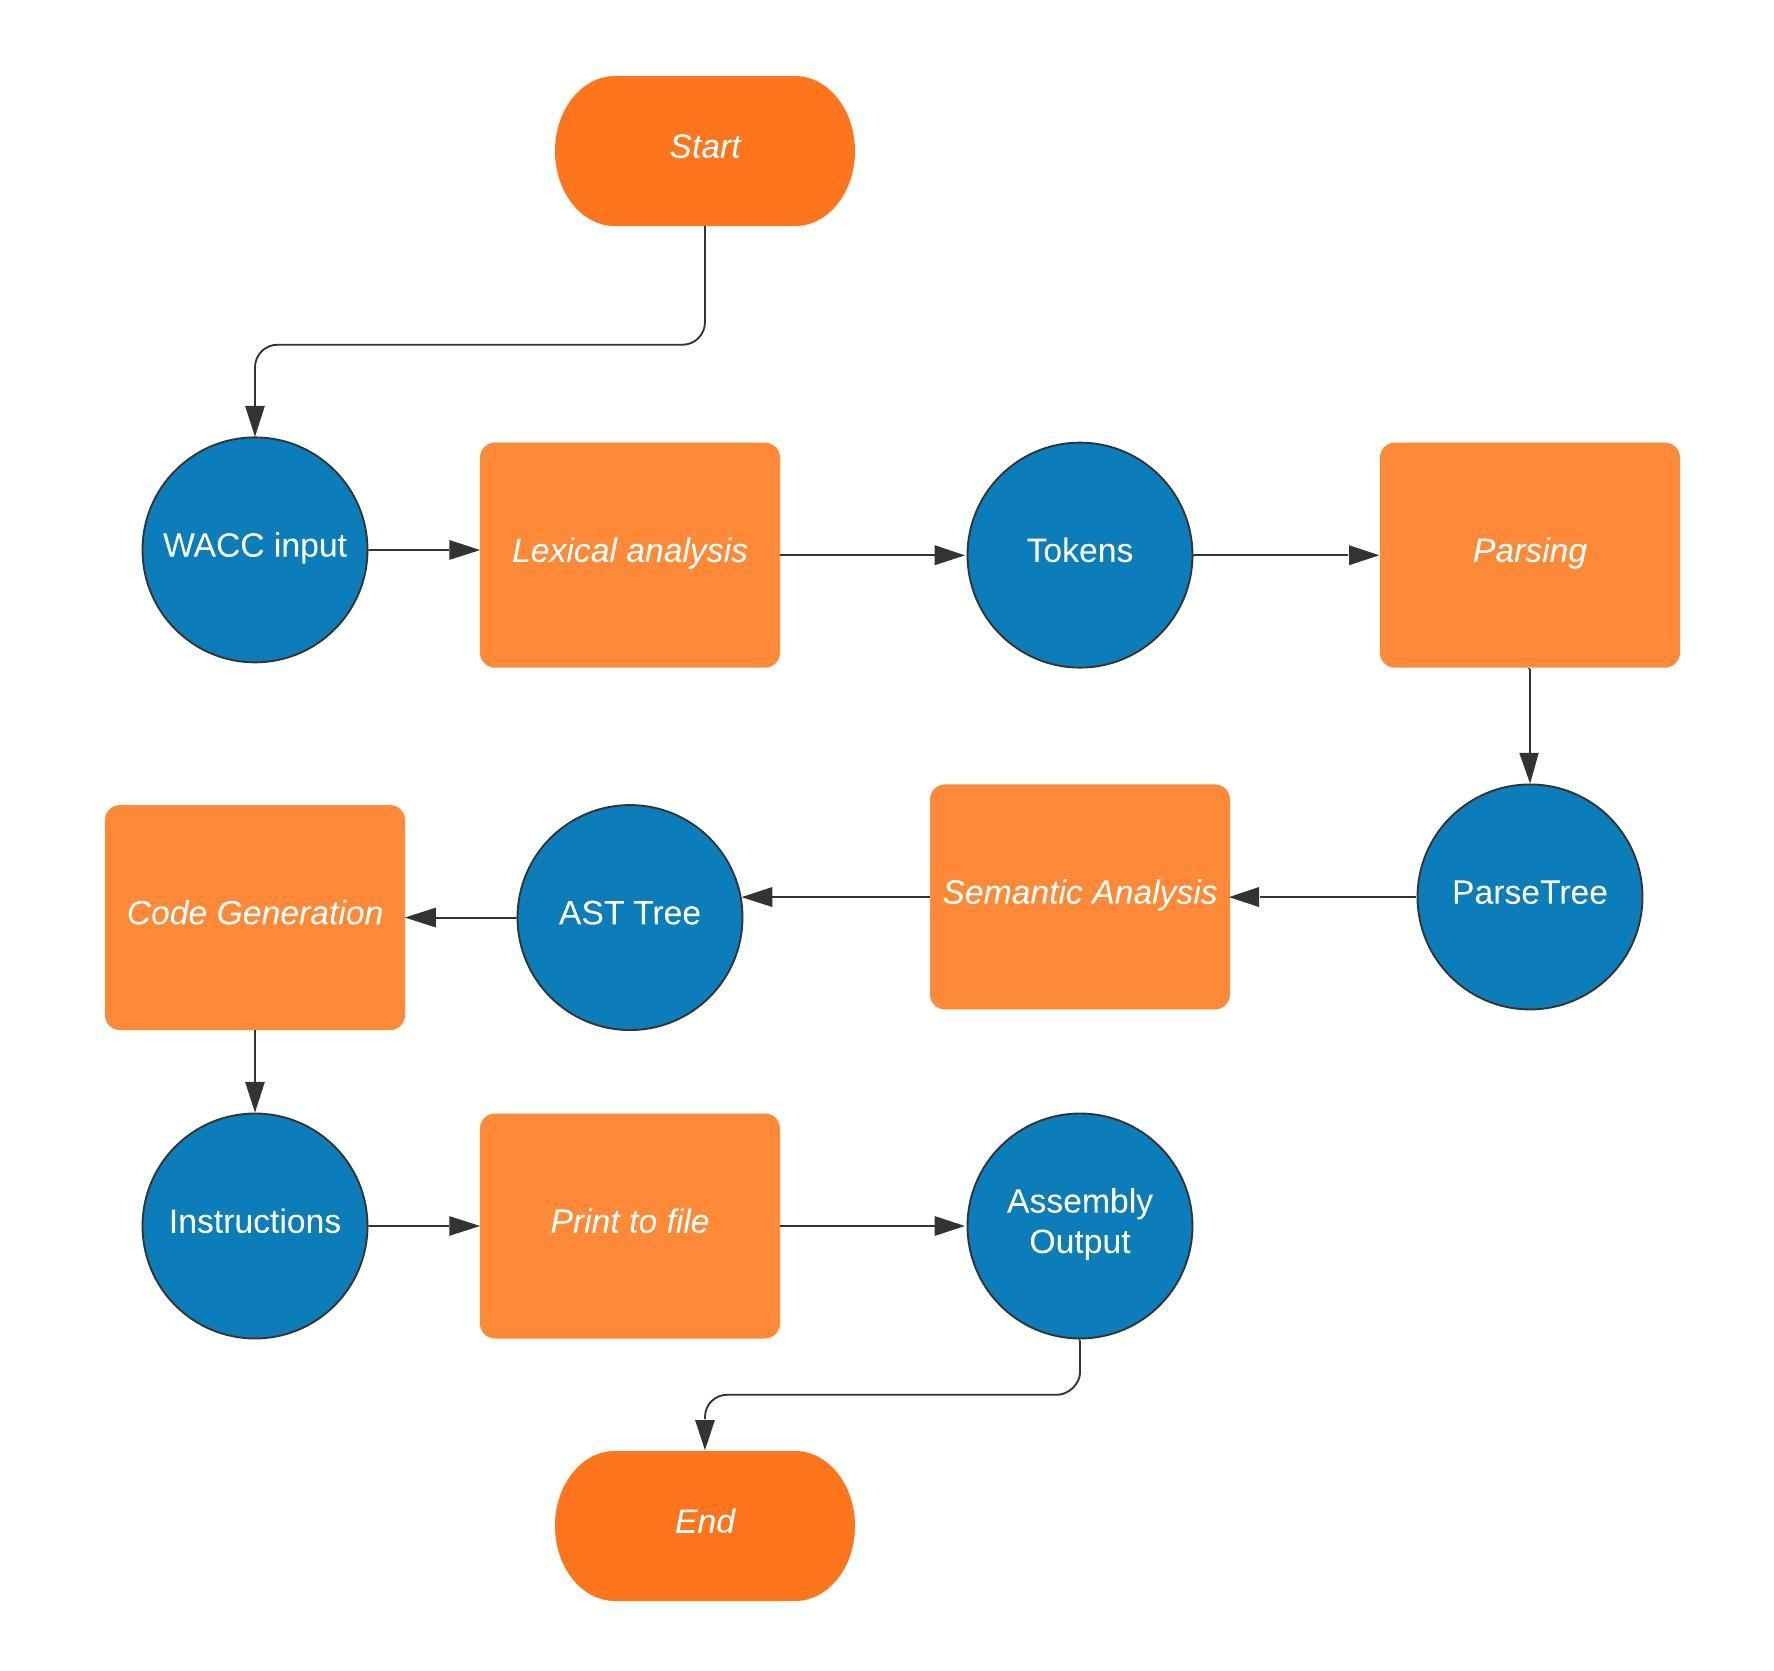
\includegraphics[width=\textwidth]{system.jpeg}
  \caption{System Architecture Diagram}
\end{figure}

\begin{table}
    \label{sec:table1}
    \begin{center}
      \begin{tabular}{|| m{10em} | m{15em} | m{15em} ||} 
      \hline
        & Variables & Functions \\
      \hline
      Able to inherit & \multicolumn{2}{C{30em}||}{YES - 
      A subclass automatically contains the variables and functions defined in its superclass, on top of any additional variables and functions defined in its own struct. 
      }\\
      \hline
      Able to override & YES - same type, NO - different type
      Subclasses are not allowed to override superclass variables by defining another variable with the same name but a different type, as methods in the superclass may operate on its variables.
      &
      YES - 
    It is possible for the subclass to override the definitions of its superclass’s functions by defining functions with the same name. The subclass can give the function a different signature (by defining it to take in different parameters).  \\
    \hline
      \end{tabular}
      \caption{Inheritance Rules}
    \end{center}

    \begin{center}
        \label{sec:table23}
        \begin{tabular}{|| m{10em} | m{15em} | m{15em} ||} 
        \hline
        Object & Able to have same name & Unable to have same name \\
        \hline
        Classes & Main class, Functions & Other classes \\
        \hline
        Class instances & Classes & Other class instances \\
        \hline
        Variables in classes & Variable outside of its class, Functions & Other variables in the same class, Parameters of functions defined in the same class \\
        \hline
        Functions in classes & Functions outside of its class or in another class & Functions defined in the same class \\
        \hline
        \end{tabular}
        \caption{Naming Rules}
    \end{center}

    \begin{center}
        \begin{tabular}{|| m{16em} | m{25em} ||} 
        \hline
        Code & Description \\
        \hline
        \cmd{Class1 c = new Class2()} & Classes can be initialized in the body of the main code by making a new class. Class1 and Class2 must be of the same class OR Class1 must be the superclass of Class2.  \\
        \hline
        \cmd{Class1 d = c} & Classes can also be initialized by assigning an existing class instance to the new class. c must be of class Class1 OR c’s class must be the subclass of Class1. \\
        \hline
        \cmd{e = c} where both e and c are class instances & An existing class instance can also be assigned to another existing class instance.
        These instances must be of the same class OR e’s class must be the superclass of c’s class. \\
        \hline        
        \end{tabular}
        \caption{Initialisation of Classes with Inheritance}
    \end{center}


\end{table}

\end{document}
